\section{Results}

\begin{table}
    \centering
    \caption{Execution time as a function of $\log n$}
    \begin{tabular}{|l|c|c|c|c|c|} \hline
        $\log n$ & SS & AKS & MR & TD & WS \\
        \hline
1 & 8 & 1726 & 13 & 12 & 8 \\
2 & 110 & 19326 & 128 & 8 & 8 \\
3 & 110 & 32415 & 130 & 14 & 16 \\
4 & 122 & 689248 & 140 & 20 & 14 \\
5 & 156 & 582623 & 184 & 23 & 18 \\
6 & 169 & 3735301 & 190 & 26 & 18 \\
7 & 192 & 10045207 & 212 & 29 & 20 \\
8 & 211 & 21503625 & 217 & 32 & 21 \\
9 & 234 & 60103404 & 237 & 36 & 22 \\
10& 254 & 127910717 & 245 & 40 & 25 \\
11& 275 & 292019772 & 256 & 46 & 27 \\
12& 297 & 581977224 & 269 & 54 & 30 \\
13& 321 & 1014476731 & 278 & 64 & 34 \\
14& 726.0 & - & 292.0 & 78.0 & 39.0 \\
15& 1278.0 & - & 304.0 & 94.0 & 44.0 \\
16& 702.0 & - & 316.0 & 117.0 & 52.0 \\
17& 749.0 & - & 330.0 & 149.0 & 63.0 \\
18& 790.0 & - & 342.0 & 189.0 & 77.0 \\
19& 830.0 & - & 354.0 & 251.0 & 94.0 \\
20& 873.0 & - & 369.0 & 325.0 & 118.0 \\
21& 914.0 & - & 382.0 & 1499.0 & 154.0 \\
22& 954.0 & - & 409.0 & 1005.0 & 513.0 \\
23& 997.0 & - & 747.0 & 1332.0 & 727.0 \\
24& 1037.0 & - & 772.0 & 1798.0 & 624.0 \\
25& 1075.0 & - & 794.0 & 2399.0 & 828.0 \\
26& 1120.0 & - & 819.0 & 3252.0 & 1112.0 \\
27& 1157.0 & - & 844.0 & 4438.0 & 1512.0 \\
28& 1197.0 & - & 871.0 & 6130.0 & 2073.0 \\
29& 1238.0 & - & 897.0 & 7479.0 & 2841.0 \\
30& 1017.0 & - & 922.0 & 11676.0 & 3915.0 \\
31& 1318.0 & - & 947.0 & 14595.0 & 5036. \\
        \hline
    \end{tabular}
\end{table}


\begin{table}
    \centering
    \caption{Error as a function of $\log n$}
    \begin{tabular}{|l|c|c|c|c|c|} \hline
        $\log n$ & SS & AKS & MR & TD & WS \\
        \hline
1 & 1.0 & 1.0 & 1.0 & 1.0 & 1.0 \\
2 & 1.0 & 1.0 & 1.0 & 1.0 & 1.0 \\
3 & 1.0 & 1.0 & 1.0 & 1.0 & 1.0 \\
4 & 0.951203 & 1.0 & 0.95053 & 1.0 & 1.0 \\
5 & 0.978582 & 1.0 & 0.978538 & 1.0 & 1.0 \\
6 & 0.983269 & 1.0 & 0.984793 & 1.0 & 1.0 \\
7 & 0.985784 & 1.0 & 0.987807 & 1.0 & 1.0 \\
8 & 0.991804 & 1.0 & 0.992822 & 1.0 & 1.0 \\
9 & 0.993558 & 1.0 & 0.99467 & 1.0 & 1.0 \\
10& 0.995892 & 1.0 & 0.996872 & 1.0 & 1.0 \\
11& 0.996757 & 1.0 & 0.997659 & 1.0 & 1.0 \\
12& 0.997884 & 1.0 & 0.998644 & 1.0 & 1.0 \\
13& 0.998752 & 1.0 & 0.999046 & 1.0 & 1.0 \\
14& 0.999077 & - & 0.999402 & 1.0 & 1.0 \\
15& 0.999396 & - & 0.999603 & 1.0 & 1.0 \\
16& 0.999572 & - & 0.999767 & 1.0 & 1.0 \\
17& 0.999736 & - & 0.999844 & 1.0 & 1.0 \\
18& 0.999832 & - & 0.999898 & 1.0 & 1.0 \\
19& 0.999872 & - & 0.999928 & 1.0 & 1.0 \\
20& 0.999923 & - & 0.999947 & 1.0 & 1.0 \\
21& 0.99994 & - & 0.999969 & 1.0 & 1.0 \\
22& 0.999975 & - & 0.999988 & 1.0 & 1.0 \\
23& 0.999971 & - & 0.999994 & 1.0 & 1.0 \\
24& 0.999983 & - & 0.99999 & 1.0 & 1.0 \\
25& 0.999991 & - & 0.999992 & 1.0 & 1.0 \\
26& 0.99999 & - & 0.999997 & 1.0 & 1.0 \\
27& 0.999996 & - & 0.999997 & 1.0 & 1.0 \\
28& 0.999996 & - & 1.0 & 1.0 & 1.0 \\
29& 0.999997 & - & 1.0 & 1.0 & 1.0 \\
30& 0.999999 & - & 1.0 & 1.0 & 1.0 \\
31& 1.0 & - & 1.0 & 1.0 & 1.0 \\
        \hline
    \end{tabular}
\end{table}

\begin{figure}
        \centering
        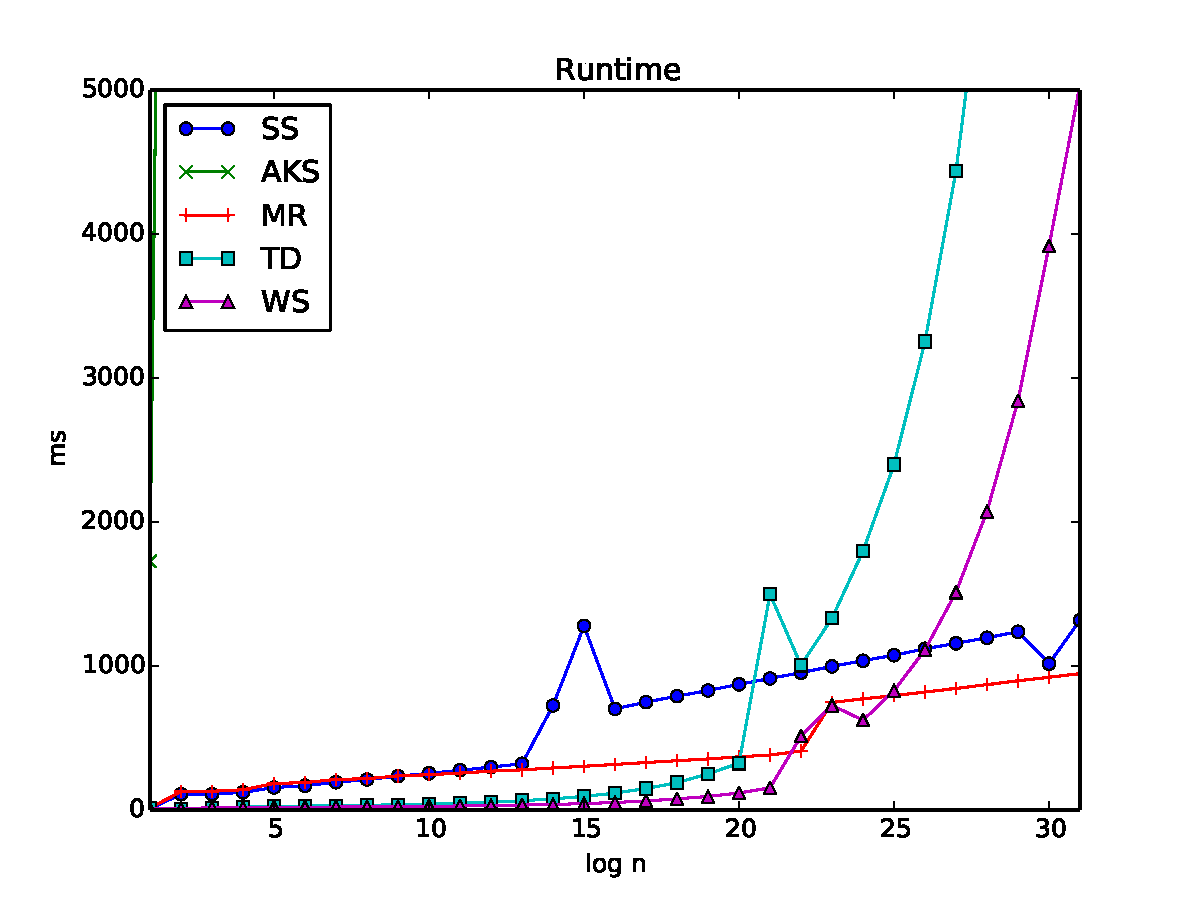
\includegraphics[width=\columnwidth]{results/runtime.pdf}
        \caption{Execution time as function of $\log n$}
        \label{fig:executionTime1}
\end{figure}

\begin{figure}
        \centering
        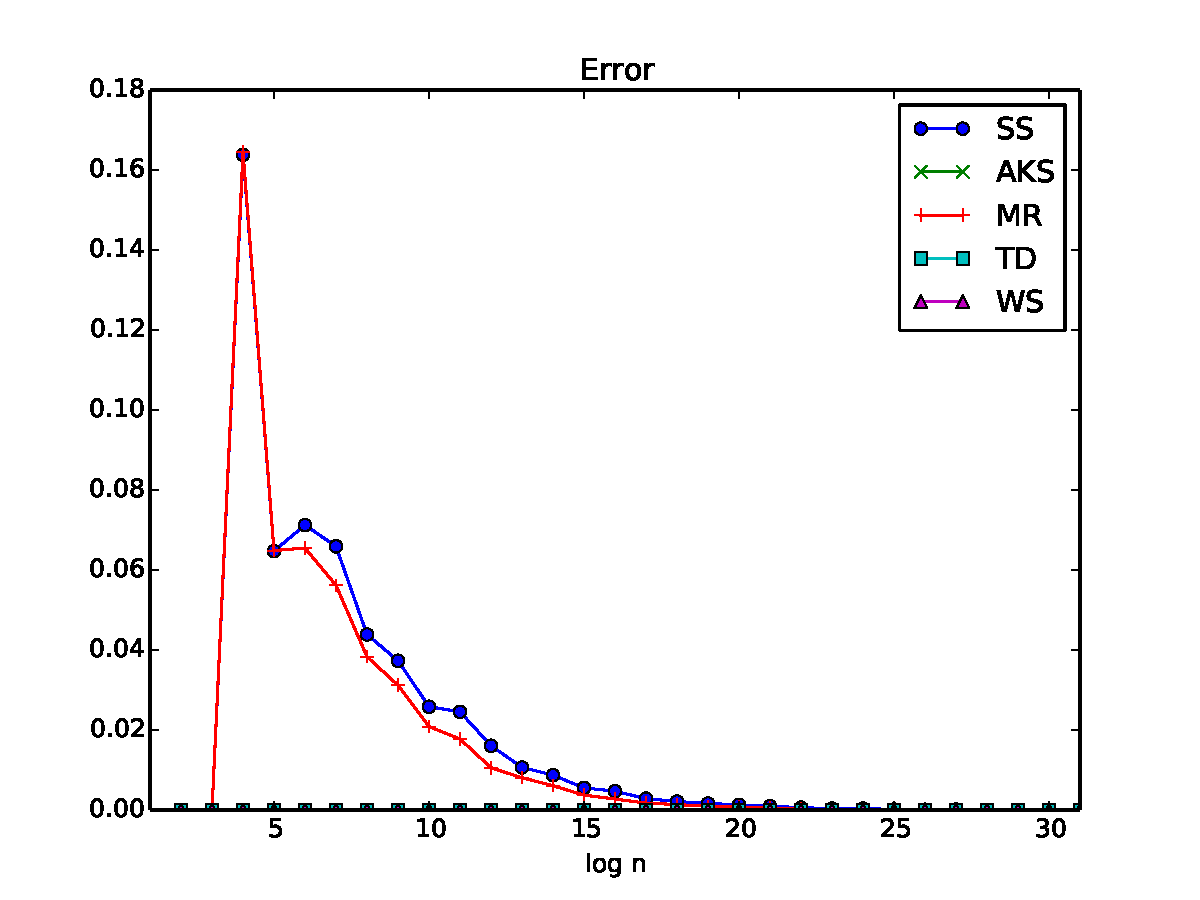
\includegraphics[width=\columnwidth]{results/performance.pdf}
        \caption{Execution time as function of $\log n$}
        \label{fig:executionTime1}
\end{figure}




%\begin{table}
%\centering
%\caption{Execution time as a function of $n$. Each datapoint consists of 10,000 samples.}
%\begin{tabular}{|l|c|c|c|c|c|} \hline
%Range\textbackslash Method&AKS&MR&SS&TD&WS \\ \hline
%2-500&6.55E9&1.86E-2&2.20E-2&3.61E-3&1.06E-2 \\ \hline
%501-5000&-&1.94E-2&2.52E-2&4.65E-3&1.26E-2 \\ \hline
%5001-50000&-&2.11E-2&2.82E-2&6.36E-3&1.44E-2 \\ \hline
%50001-500000&-&2.19E-2&3.15E-2&1.03E-2&1.74E-2 \\ \hline
%\end{tabular}
%\label{tab:pressure}
%\end{table}




%\begin{table}
%\centering
%\caption{Error (fraction) as a function of $n$. Each datapoint consists of 10,000 samples. All methods have a one-sided error: they may say ``prime'', while it is a composite.}
%\begin{tabular}{|l|c|c|c|c|c|} \hline
%Range\textbackslash Method&AKS&MR&SS&TD&WS \\ \hline
%2-500&0&1.27E-2&9.52E-3&0&0 \\ \hline
%501-5000&-&2.64E-3&2.99E-3&0&0 \\ \hline
%5001-50000&-&1.11E-3&5.53E-4&0&0 \\ \hline
%50001-500000&-&1.09E-4&0&0&0 \\ \hline
%\end{tabular}
%\label{tab:pressure}
%\end{table}



%\begin{figure}
        %\centering
        %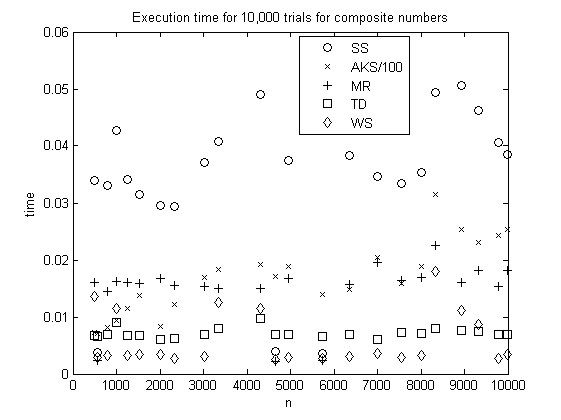
\includegraphics[width=0.5\textwidth]{../Graphs/ExecutionTime1.png}
        %\caption{Execution time for small composite numbers, $n$. Each measurement consists of 10,000 samples.}
        %\label{fig:executionTime1}
%\end{figure}


%\begin{figure}
        %\centering
        %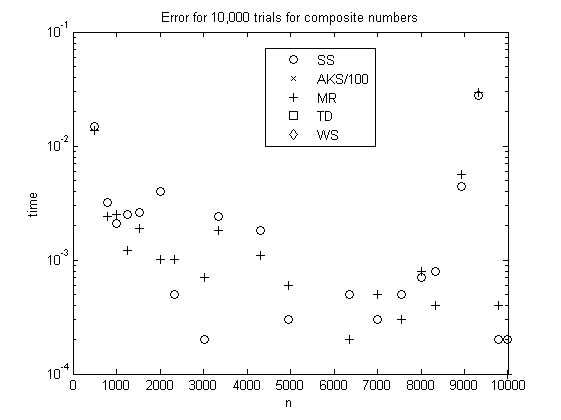
\includegraphics[width=0.5\textwidth]{../Graphs/Error1.png}
        %\caption{Error (false prime prediction) for small composite numbers, $n$. Each measurement consists of 10,000 samples.}
        %\label{fig:error1}
%\end{figure}


%\begin{figure}
        %\centering
        %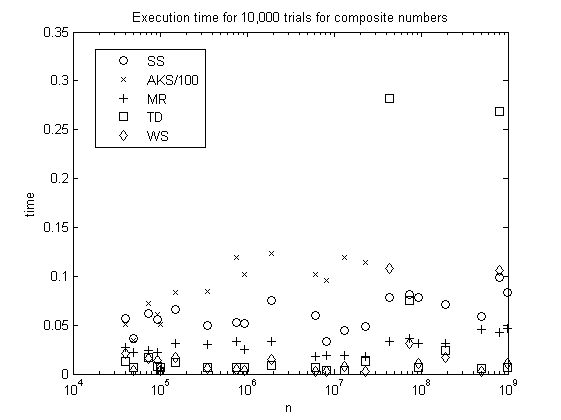
\includegraphics[width=0.5\textwidth]{../Graphs/ExecutionTime2.png}
        %\caption{Execution time for a large range of composite numbers, $n$. Each measurement consists of 10,000 samples.}
        %\label{fig:executionTime2}
%\end{figure}



%\begin{figure}
        %\centering
        %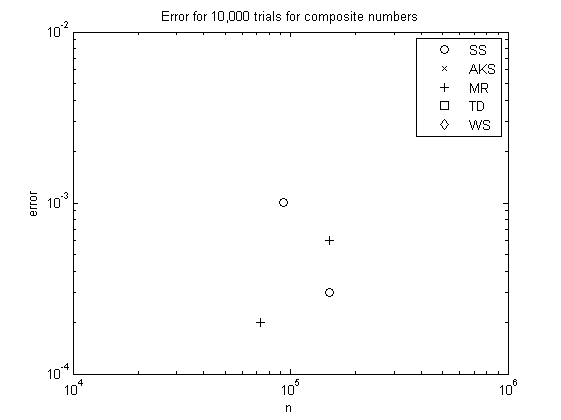
\includegraphics[width=0.5\textwidth]{../Graphs/Error2.png}
        %\caption{Error (false prime prediction) for a large range of composite numbers, $n$. Each measurement consists of 10,000 samples.}
        %\label{fig:error2}
%\end{figure}

